\chapter{Darla}
Two months had passed since I first casted Adrienne, and it's been a great two months.

A few days ago, I went downstairs to check my stash of removed casts: 13 casts worn by 6
beautiful women in ten weeks. Pretty good, for a guy who never casted a woman before.

I faced a bit of a dilemma though- Spring semester was nearly over. I was concerned that
between students heading home for the summer, and some getting jobs, I might not have many
potential models around to cast.

But, that particular day, I had an interview with a potential model. Her name was Darla, and
she was due to arrive within the hour.

Darla was right on time. She was a tall brunette with unbelievably beautiful eyes. Of
course, the rest of her looked fantastic, too, but her eyes were an icy shade of blue with a
definite hint of mischief in them.

In the parlor, I explained the job to her, outlined the process, and told her what the pay
would be. She seemed a bit reluctant, probably surprised by the weirdness of what I was
proposing. In the end, she decided to go through with it. I gave her some basic wardrobe
options, and we agreed to meet on Friday afternoon at 2:00 p.m. for our session.

Friday rolled around, and at 2:00, Darla arrived right on time. She wore denim shorts, a
black T-shirt and white sneakers. She looked really good in street clothes, and was about to
look much better in fiberglass.

I led her to the casting room, and pre-paid her as I do all of my models. As she put the
envelope away, I asked what she'd brought to wear. She opened her overnight bag and produced a
long blue nightgown that looked both sexy and elegant. I had planned to cast her in pink
fiberglass, but when I had seen the gown, I changed my mind. Having plenty of supplies on hand,
changes like this were always possible. The gown would be better accented by blue fiberglass, so
I went to retrieve a box of blue fiberglass while she changed.

When I returned to the casting room, Darla was seated on the table with her gown pulled up
to expose her legs. I noticed that she had underwear on that matched the gown. She looked
fantastic. I was definitely looking forward to this. I retrieved my bucket of warm water, and
set it close at hand.

I took a roll of 4-inch stockinette and unrolled about 50 inches of the soft, white
material, then cut it off. ``If you're ready, we'll get started,'' I said.

``Sure- the sooner it's begun, the sooner it's done,'' she replied, reminding me that I was
probably the only one in the room who would enjoy this. To her it was only a job, as she
believed it to be for me, as well.

I slid the stockinette up her right leg to the upper thigh. I maintained my usual level of
professionalism as I touched her, and I noticed a slight tensing in her muscles as my hands were
on her thigh.

I continued with a roll of 6-inch padding. I began wrapping her thigh from the top,
overlapping the turns by one half, so that as I worked, I put an even two layers of padding on
the leg. As I wrapped the padding over her knee, I added a third layer to protect the bones that
protrude around the joint. I then tore the roll of padding, and pressed the end down. I switched
to 4-inch padding for the lower leg and foot. I wrapped the rest of her leg and foot in two
layers of the soft material, with an extra layer around the ankle.

I then cut a shorter length of stockinette, and placed it on her left leg, stopping just
past the knee. Another roll of 4 inch padding gave her left leg the required thickness of
padding, and the fact that I worked downwards reduced the bunching effect you can get if you
wrap upwards with padding or casting tape.

Her legs look great. I always love the way a cast in progress looks at this point: her legs
are thick with soft white padding, and the anticipation of the hard shell soon to cover them is
a great feeling.

As I removed the first roll of 4-inch medium blue fiberglass from the box, and tore open the
foil wrapping, I informed her that the fiberglass would get warm as it set, but that the heat
would quickly dissipate before it got unbearable. I dipped the first roll, and began encasing
her left leg just below the knee. I overlapped the turns of fiberglass by thirds, so that I put
a uniform layer of fiberglass on her leg. This roll ended near her foot and the second one
started where it left off. By the time these two rolls were applied, her lower leg was covered
from knee to toes in blue fiberglass, and all that remained was to fold back the edges of
stockinette and padding, and apply one more roll of fiberglass over the entire cast to anchor
them. It sort of surprised me how quickly this cast was complete, but it looked very good, so I
assumed that the speed was simply a result of my improving techniques. As I placed her casted
leg on a stand to dry, I noticed the telltale droplets of water on the surface of the cast,
indication that it was rapidly setting.

``Darla, that will be dry very soon- before we finish the other leg, actually. This won't
take long at all.'' I told her.

``That's fine,'' she said. ``Take as long as you need. I'm being paid far too well to
complain.''

I smiled and started on the other leg.

It took nearly 20 minutes and six rolls of fiberglass to encase her right leg in fiberglass
from her toes to nearly her hip. On every roll except the final roll that anchored the
stockinette and padding at the toes, I again worked from top to bottom, avoiding bunching of the
fiberglass tape. By the time the last roll was finished, the rapidly drying thigh area was
sweating out the droplets of water, indicating the heat of the exothermic setting of the
fiberglass.

``There we are. All finished with this part.'' I said. ``Just a few minutes to set, and we
can finish.''

We chatted for about 15 minutes as the casts set. I used a cloth to wipe away the droplets
of water as they appeared.

When I was satisfied that the casts were set enough to move her, I quickly tested her blood
circulation by pinching her toenails, and observing the capillary refill time, which was quick.
Good, that means the casts are not too tight. I helped her into the wheelchair, adjusted the leg
rests to accommodate her casts, and wheeled her outside to the back yard by the pool.

We experimented with poses, and she seemed to really come alive at this point, as though
posing for a camera was second nature to her. (Or maybe something she had experience with) She
tried one pose sitting sideways on the ledge around the pool with her legs crossed, and that one
struck me as wonderful. As I sketched her in that position, I tried to convey the beauty of her
eyes in the sketch, and didn't do too bad at it. When I had finished, I helped her back into the
wheelchair, and rolled her back to the casting room.

As I was cutting through the casts down each side to free her legs, I couldn't help but
notice that something about this was unsatisfying. I wasn't sure exactly what, but it seemed to
be ending too soon. She'd worn the casts, and looked great in them. I had enjoyed every part of
the process, from application to removal, but there was something more I wanted, though I wasn't
sure exactly what that might be. Was it more casts per model? Bigger casts? Less glamorous
poses, maybe something more realistic looking, maybe even with crutches or a hospital bed?

I wasn't sure what I was wanting, what next level I needed to achieve. I pondered this as I
left Darla to get dressed.

As Darla and I said our good-byes, the question still tickled my brain. I didn't know what,
but I knew I wanted more. Figuring out what the more was would be the mystery to solve.

\begin{center}
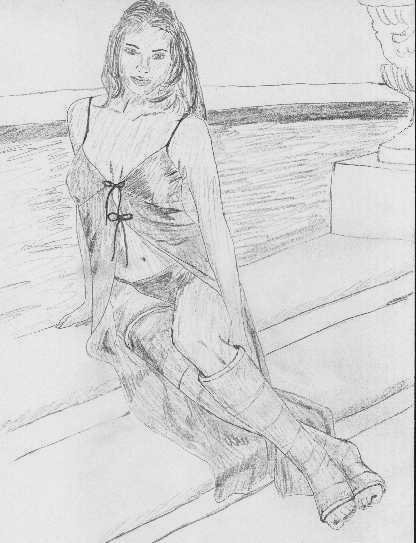
\includegraphics{images/kicks13.jpg}
\end{center}
